%!TEX root = ../../main.tex
\section{Results}
\label{sec:Results}

\subsection{Experiment 1}
\label{sub:Experiment 1 - Results}
Figure~\ref{fig:Main radioprotectant plot - Rebecca data} shows the results of the logistic curve fits to the fidelity data plotted in Figure~\ref{fig:Rebecca data}. The five-pointed stars are the points where the fitted logistic curves reach a fidelity value of 0.71. This was an arbitrary value chosen because all samples reached that value. The six-pointed stars are the maximum curvature points of the fitted logistic curves. To compare the efficacies of each radioprotectant compound, the dose at which these points occur are plotted for each scavenger in Figure~\ref{fig:Combined Scavenger results - Rebecca data}.

\begin{figure}
    \centering
    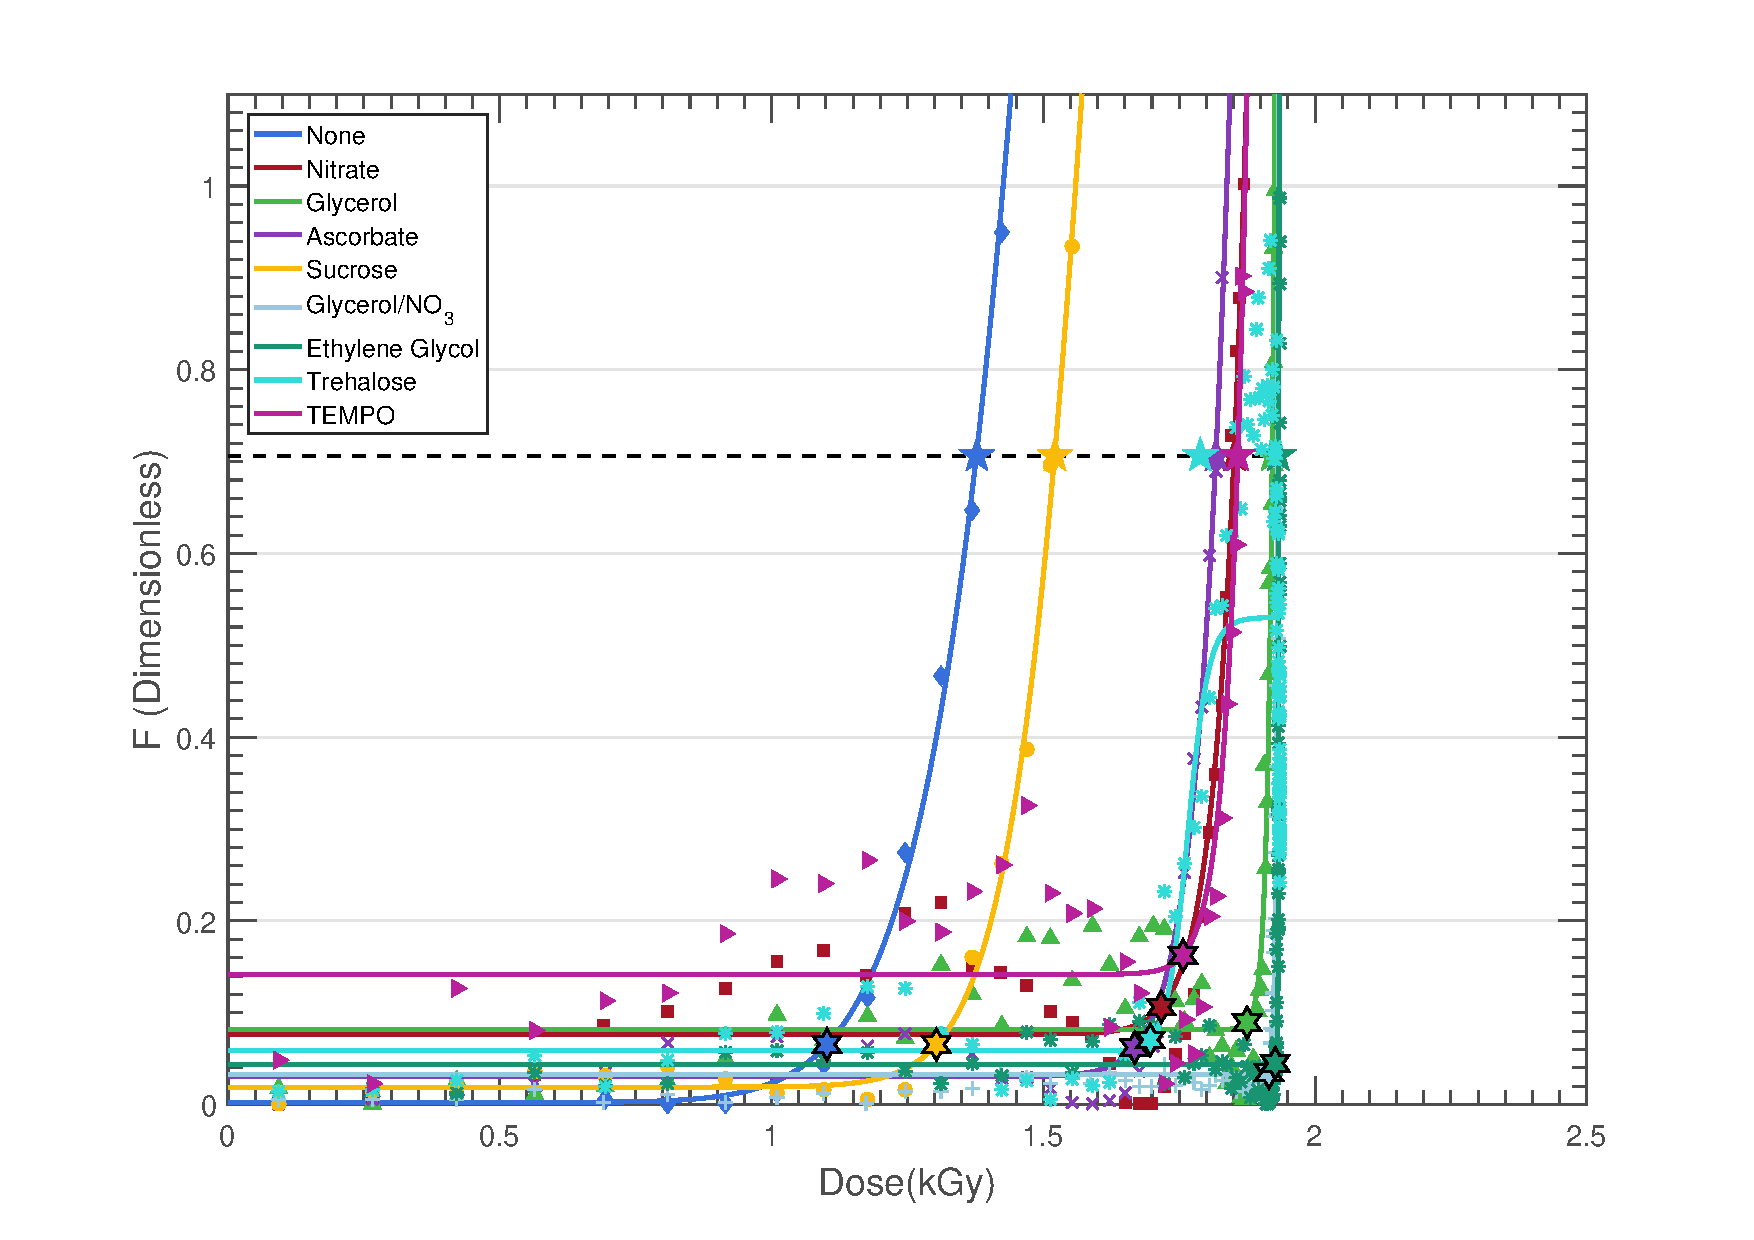
\includegraphics[width=1.0\textwidth]{figures/saxs/ScavengerPlot.pdf}
    \caption[Fidelity values as a function of dose for each radioprotectant]{Fidelity values against dose for each radioprotectant along with their corresponding fitted logistic curves. The five-pointed stars represent the points where the fitted logistic curves reach a fidelity value of 0.71. The six-pointed stars are the maximum curvature points of the fitted curves.}
    \label{fig:Main radioprotectant plot - Rebecca data}
\end{figure}

Figure~\ref{fig:Scavenger plot - arbitrary fidelity value} shows the dose taken to reach a fidelity value of 0.71 for each scavenger. Ethylene glycol is the most effective radioprotectant at 5$\,$mM concentration, closely followed by the glycerol/sodium nitrate mixture and then glycerol alone. It is clear from these results that adding a radioprotectant allows useable data to be collected for longer because the sample is less sensitive to irradiation.

Similar conclusions are obtained from Figure~\ref{fig:Scavenger plot - maximum curvature} where the dose at which maximum curvature is reached is plotted for each radioprotectant. Again ethylene glycol is shown to be the most effective radioprotectant at 5\,mM concentration, followed by the glycerol/sodium nitrate mixture and then glycerol alone. The only difference in the ordering of the relative efficacies of the radioprotectants between the two plots is that trehalose is more effective than ascorbate when using the maximum curvature metric, whereas the opposite is true when using the time to reach a fidelity of 0.71 metric.
This illustrates that there is sensitivity of results to the chosen metric.
\begin{figure}
    \centering
    \begin{subfigure}[b]{1.0\textwidth}
            \centering
            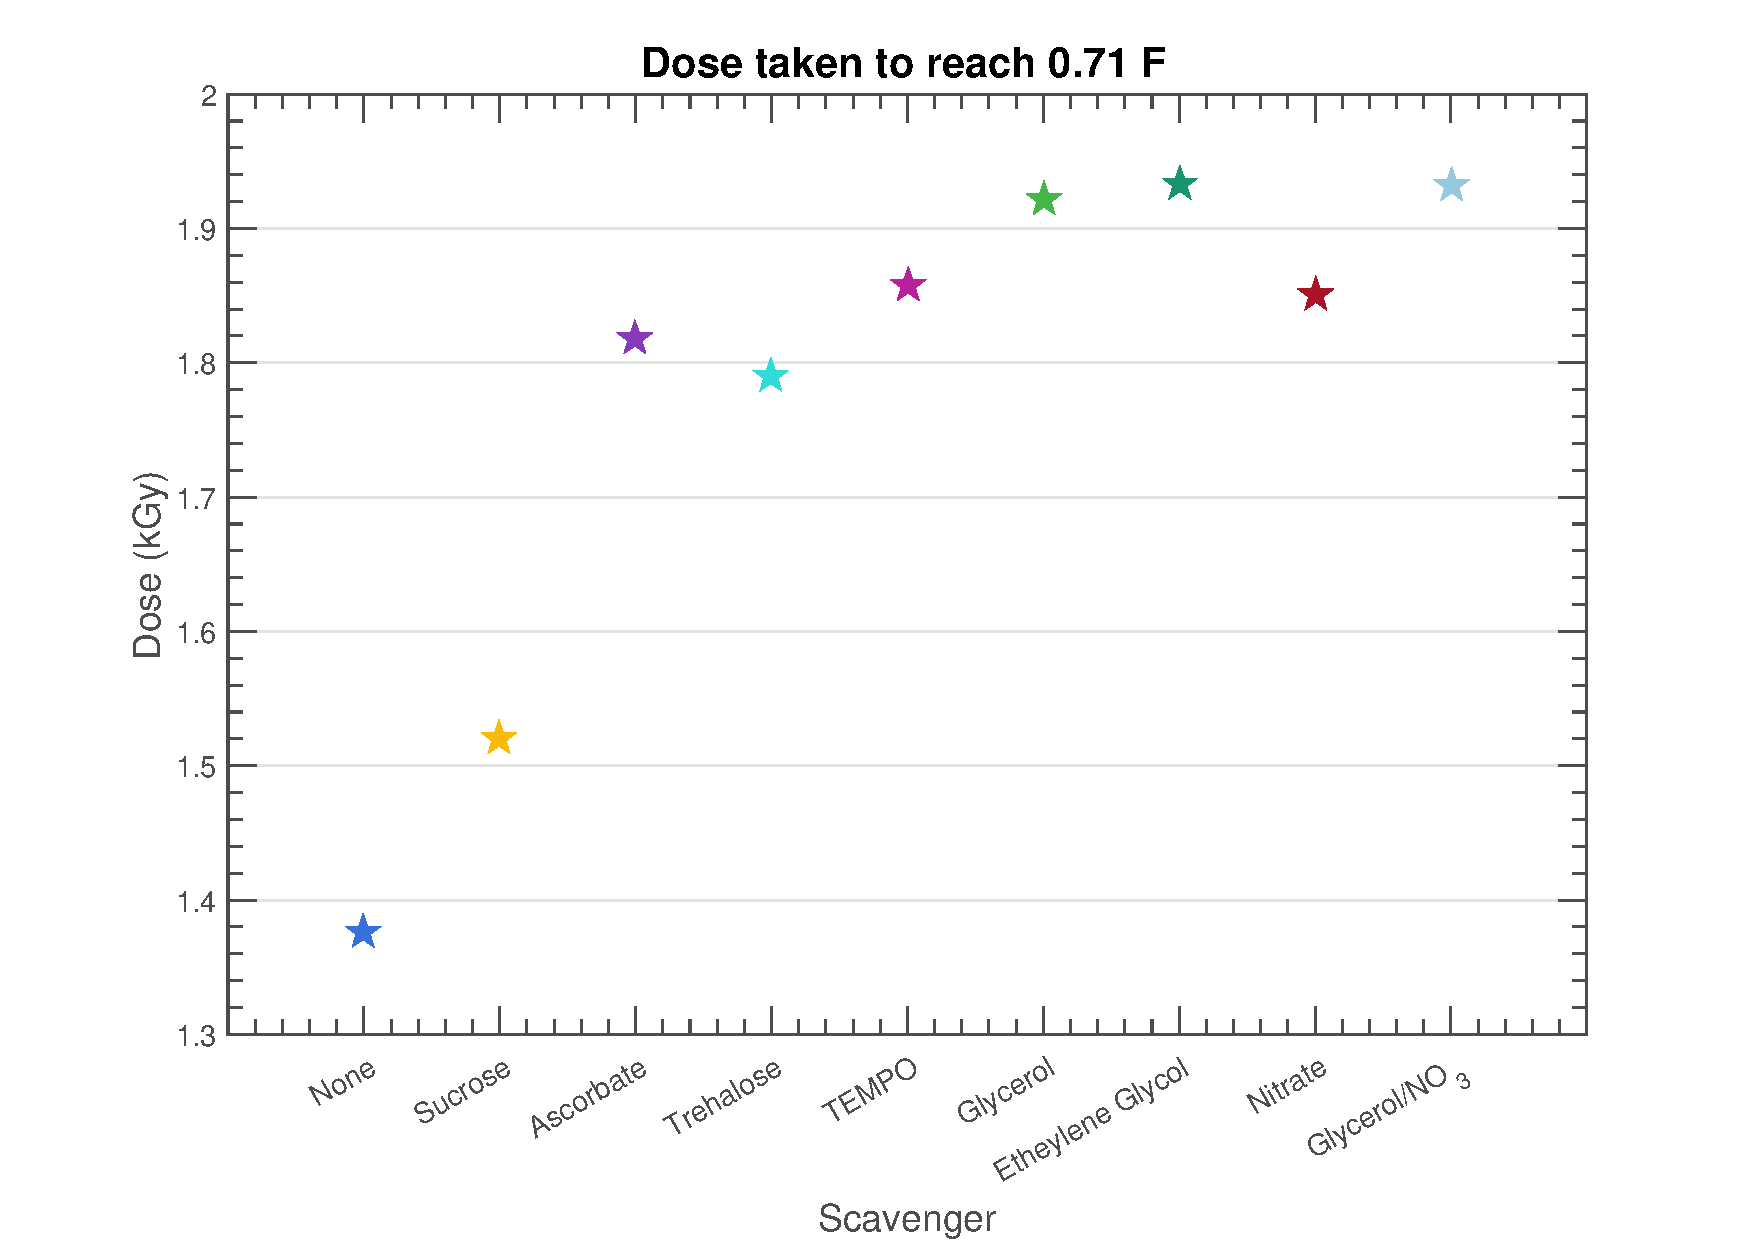
\includegraphics[width=\textwidth]{figures/saxs/ScavengerComparisonPlot.pdf}
            \caption{Expt 1: Dose taken to reach a fidelity value of 0.71 for each scavenger.}
            \label{fig:Scavenger plot - arbitrary fidelity value}
    \end{subfigure}
    \\
    \begin{subfigure}[b]{1.0\textwidth}
            \centering
            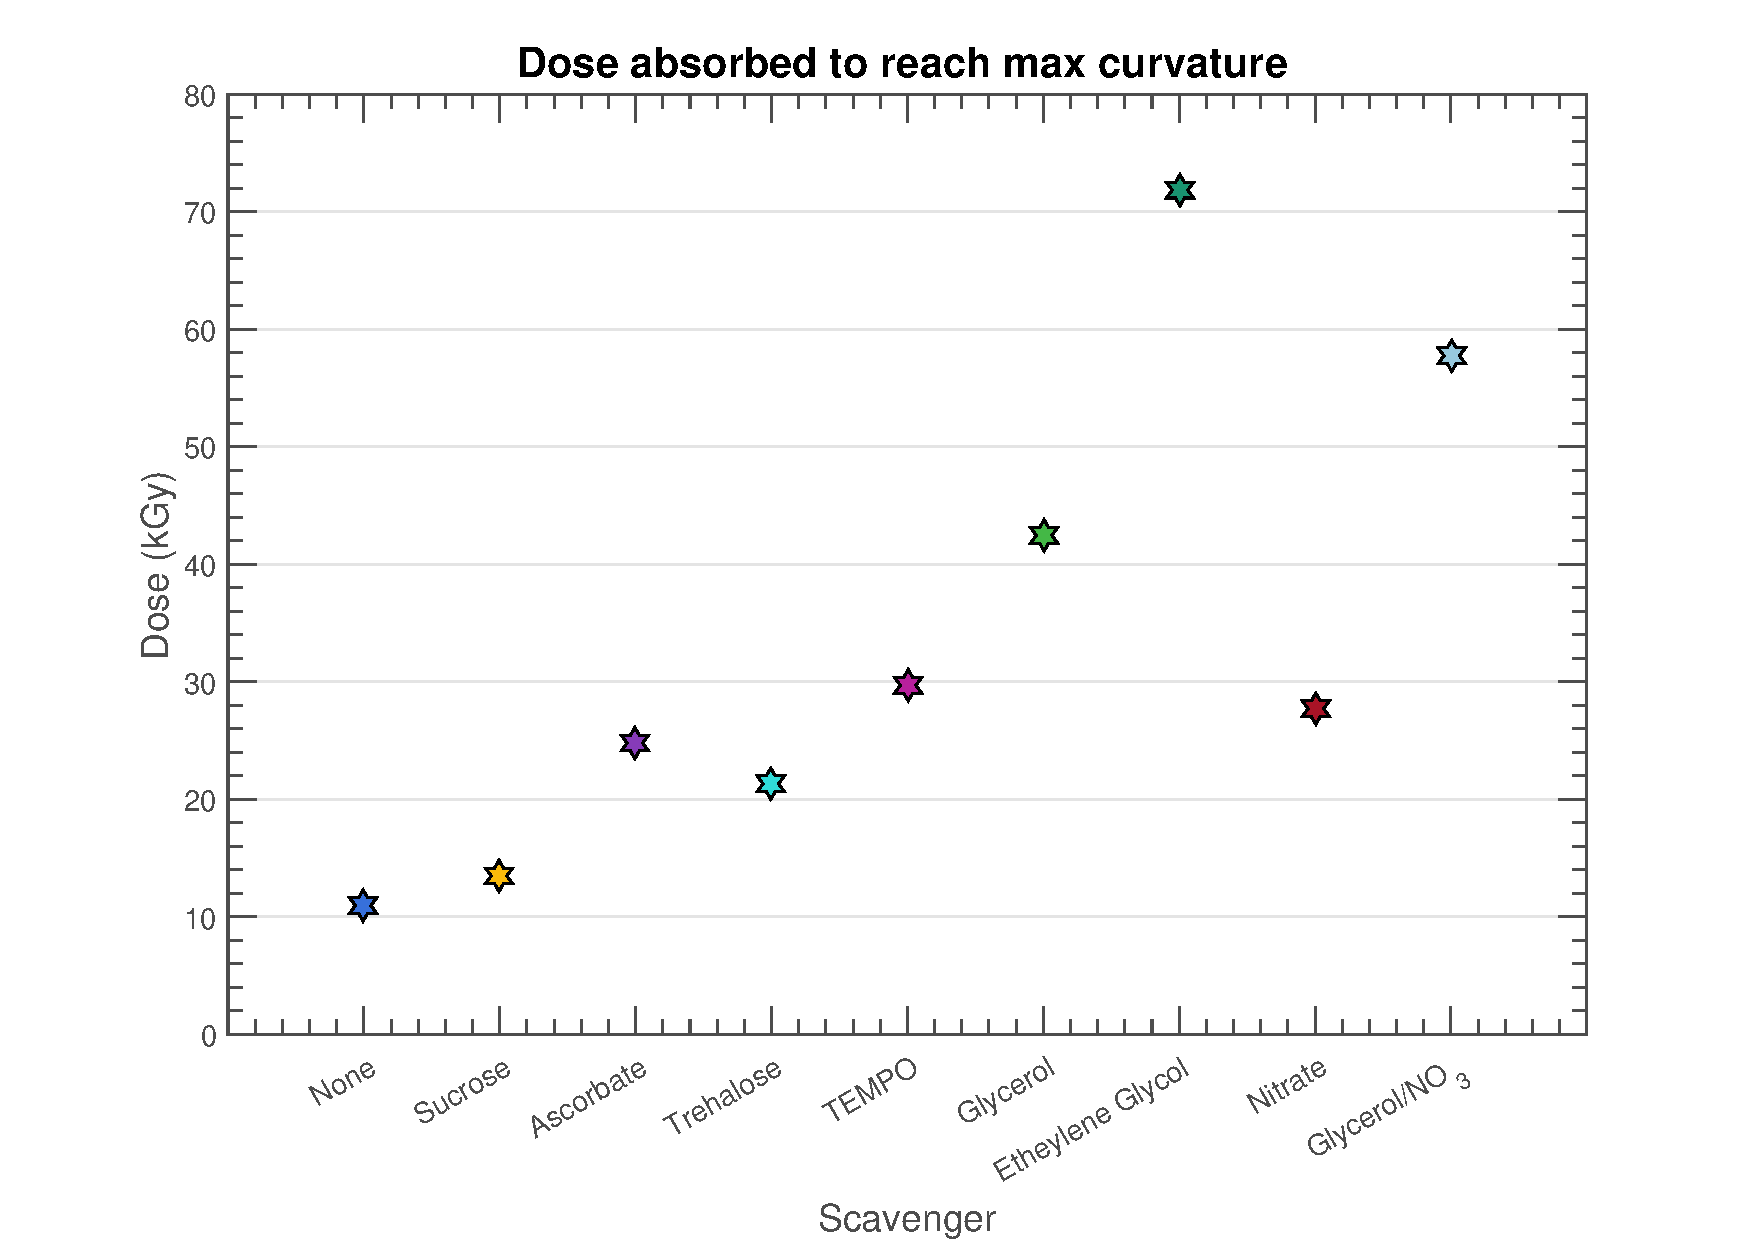
\includegraphics[width=\textwidth]{figures/saxs/ScavengerCurvatureComparisonPlot.pdf}
            \caption{Expt 1: Dose at which maximum curvature is reached}
            \label{fig:Scavenger plot - maximum curvature}
    \end{subfigure}
    \caption[Radiation damage onset threshold dose values for both metrics used to assess the fidelity values.]{}
    \label{fig:Combined Scavenger results - Rebecca data}
\end{figure}

\subsection{Experiment 2}
\label{sub:Experiment 2 - Results}

\subsubsection{Comparing radiation damage onset metrics}
\label{subs:Comparing radiation damage onset metrics}
In section \ref{sub:Data analysis - experiment 2} a metric for assessing the frame at which radiation damage had become significant was presented based on the CorMap test.
Explicitly, this metric was defined as the point at which three consecutive frames were defined as dissimilar ($m$ = 3) resulting from the CorMap test with threshold $\alpha$ = 0.01.
This metric will be referred to as the \textit{CMD} (CorMap Derived) metric.

In addition to the \textit{CMD} metric, an automatic data analysis pipeline at beamline BM29 \cite{brennich2016online} is integrated into the beamline control system, \textit{BsxCuBE}.
This pipeline additionally performs analysis of frames and hence gives merging thresholds calculated for radiation damage onset using a metric henceforth denoted the \textit{BsxCuBE} metric.

The results from analysis with both metrics were calculated/recorded and figure~\ref{fig:SAXS Metric comparison} shows how the two metrics compare for each compound at all concentrations.
Generally the two metrics agree on the order of the efficacy of the various radioprotectant compounds, but the \textit{BsxCuBE} metric always suggests that more frames can be merged then the \textit{CMD} metric.
Given that the \textit{CMD} metric was developed to avoid individual dissimilar frames prematurely being flagged as the point of significant radiation damage onset, this result is quite surprising.
It suggests that the \textit{BsxCuBE} metric employs a very different method to assess the similarity of frames than the \textit{CMD} metric.
\textcolor{red}{
    \begin{myenumerate}
        \item \hypertarget{todo:Ask Adam about BsxCuBE}{\textbf{TODO:} ask adam about the BsxCuBE metric.}
        The paper suggest that it too uses the CorMap method with the same $\alpha$ = 0.01 but the results don't match up.
    \end{myenumerate}
}
\begin{figure}
    \centering
    \begin{subfigure}[b]{0.45\textwidth}
            \centering
            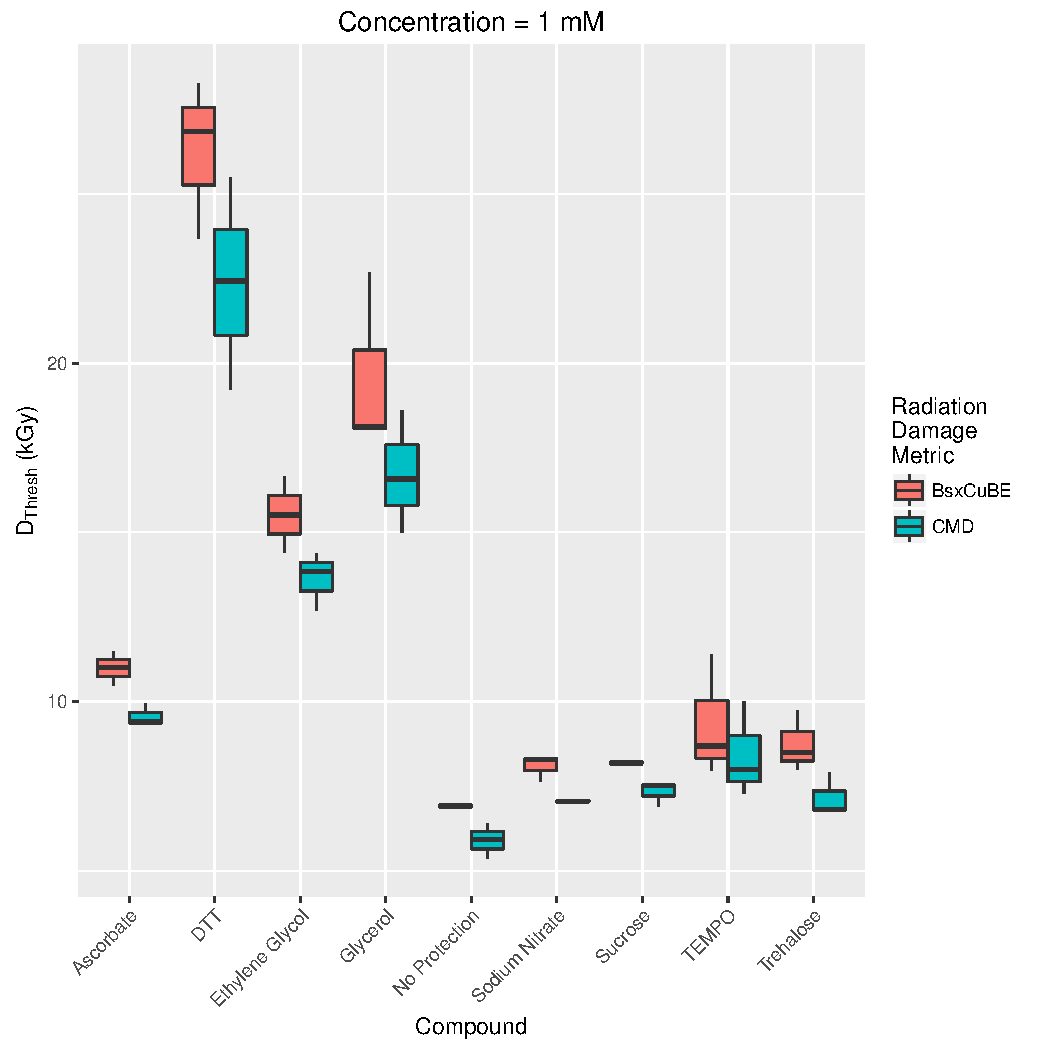
\includegraphics[width=\textwidth]{figures/saxs/Conc_1_dose.pdf}
            \caption{}
            \label{fig:SAXS Metric comparison - 1mM}
    \end{subfigure}
    \qquad
    \begin{subfigure}[b]{0.45\textwidth}
            \centering
            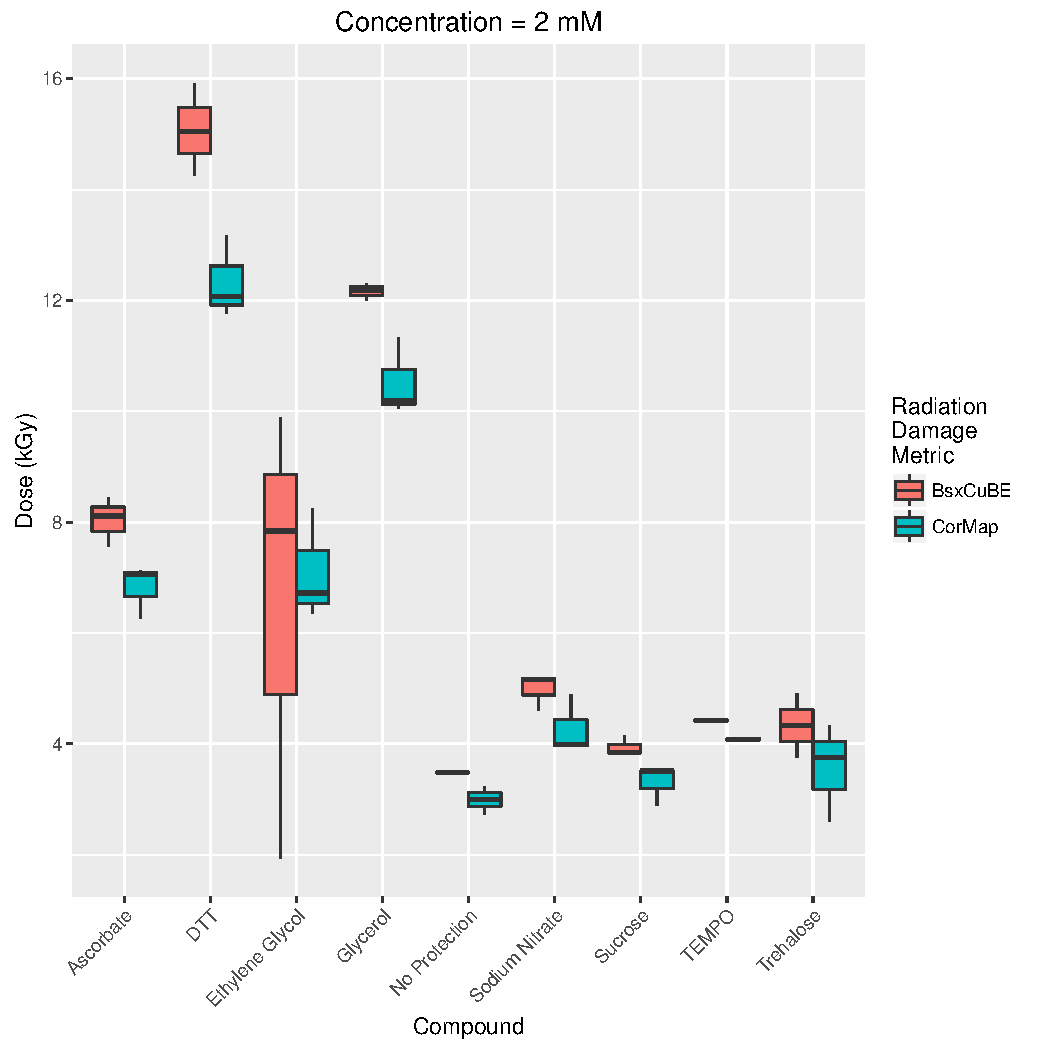
\includegraphics[width=\textwidth]{figures/saxs/Conc_2_dose.pdf}
            \caption{}
            \label{fig:SAXS Metric comparison - 2mM}
    \end{subfigure}
    \\
    \begin{subfigure}[b]{0.45\textwidth}
            \centering
            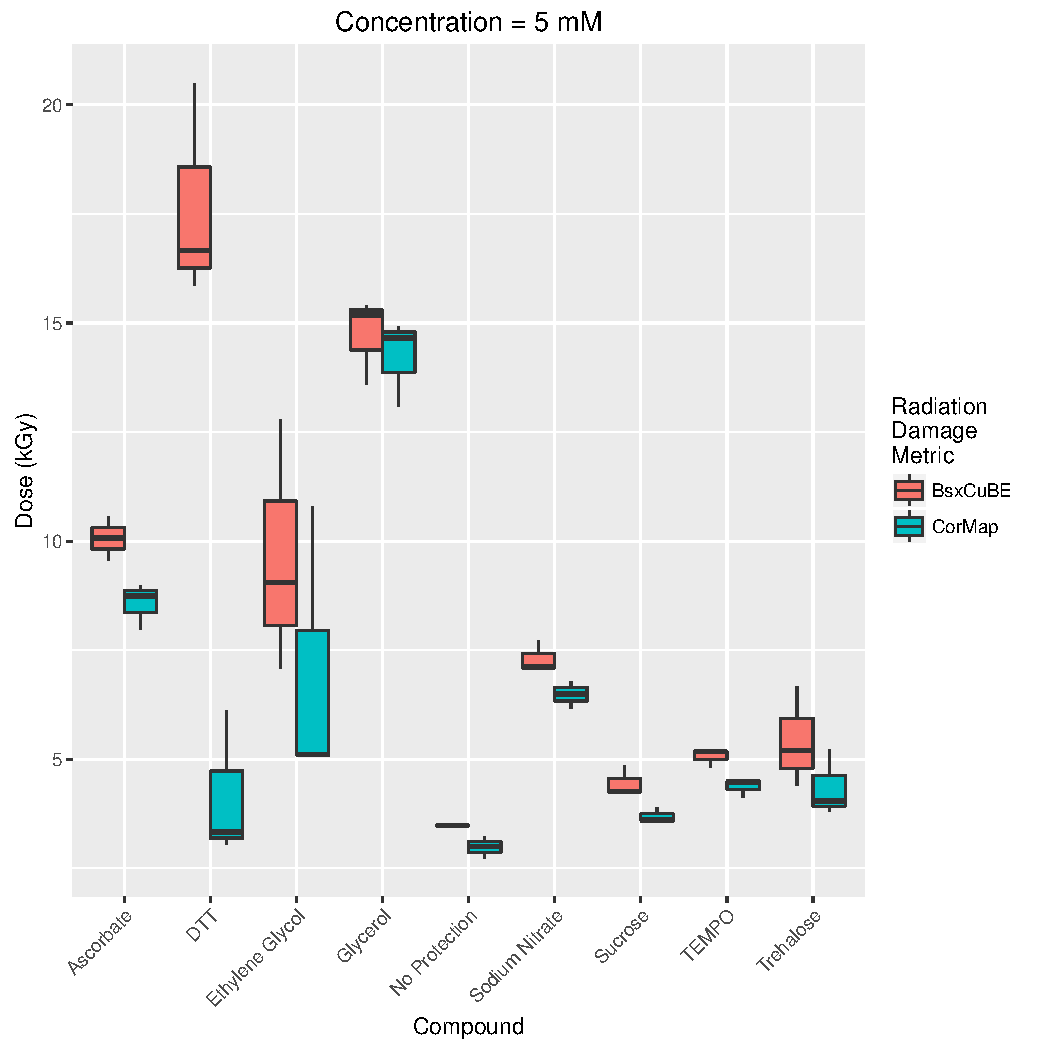
\includegraphics[width=\textwidth]{figures/saxs/Conc_5_dose.pdf}
            \caption{}
            \label{fig:SAXS Metric comparison - 5mM}
    \end{subfigure}
    \qquad
    \begin{subfigure}[b]{0.45\textwidth}
            \centering
            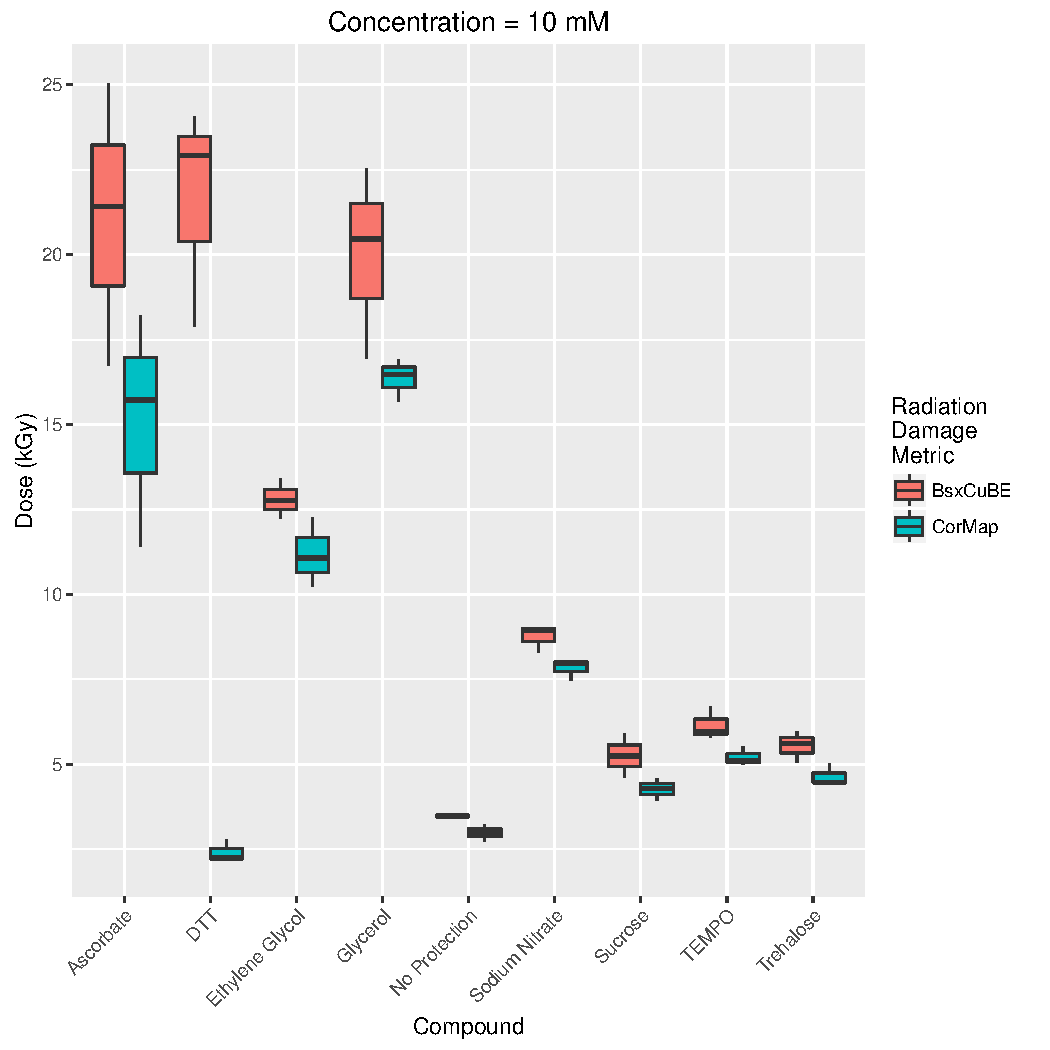
\includegraphics[width=\textwidth]{figures/saxs/Conc_10_dose.pdf}
            \caption{}
            \label{fig:SAXS Metric comparison - 10mM}
    \end{subfigure}
    \caption[Radioprotectant efficacy comparison  boxplots for each concentration in the experiment.]{Dose value at which radiation damage is considered significant. Each box plot is created from the threshold dose values calculated for three different experimental runs of the same radioprotectant compound. Pink boxes correspond to the \textit{BsxCuBE} metric, blue boxes correspond to the \textit{CMD} metric}
    \label{fig:SAXS Metric comparison}
\end{figure}

The biggest discrepancy between the two metrics is the result for DTT.
The \textit{BsxCuBE} metric predicts a much higher dose tolerance than the \textit{CMD} metric, especially for the 5$\,$mM and 10$\,$mM concentrations.
One reason thought to cause this discrepancy in the current work was the choice of $m$ = 3 for the \textit{CMD} metric.
Figure~\ref{fig:Num consec frames - DTT} shows the results of the various values of $m$ for DTT.
Unlike the results for ascorbate (Figure~\ref{fig:Num consecutive frame test}) and the other compounds, the chosen value of $m$ could be the problem for 5$\,$mM concentrations.
However, this does not necessarily seem to be true for the 10$\,$mM concentration.
Thus it was necessary to re-evaluate some of the underlying assumptions.
\begin{figure}
    \centering
    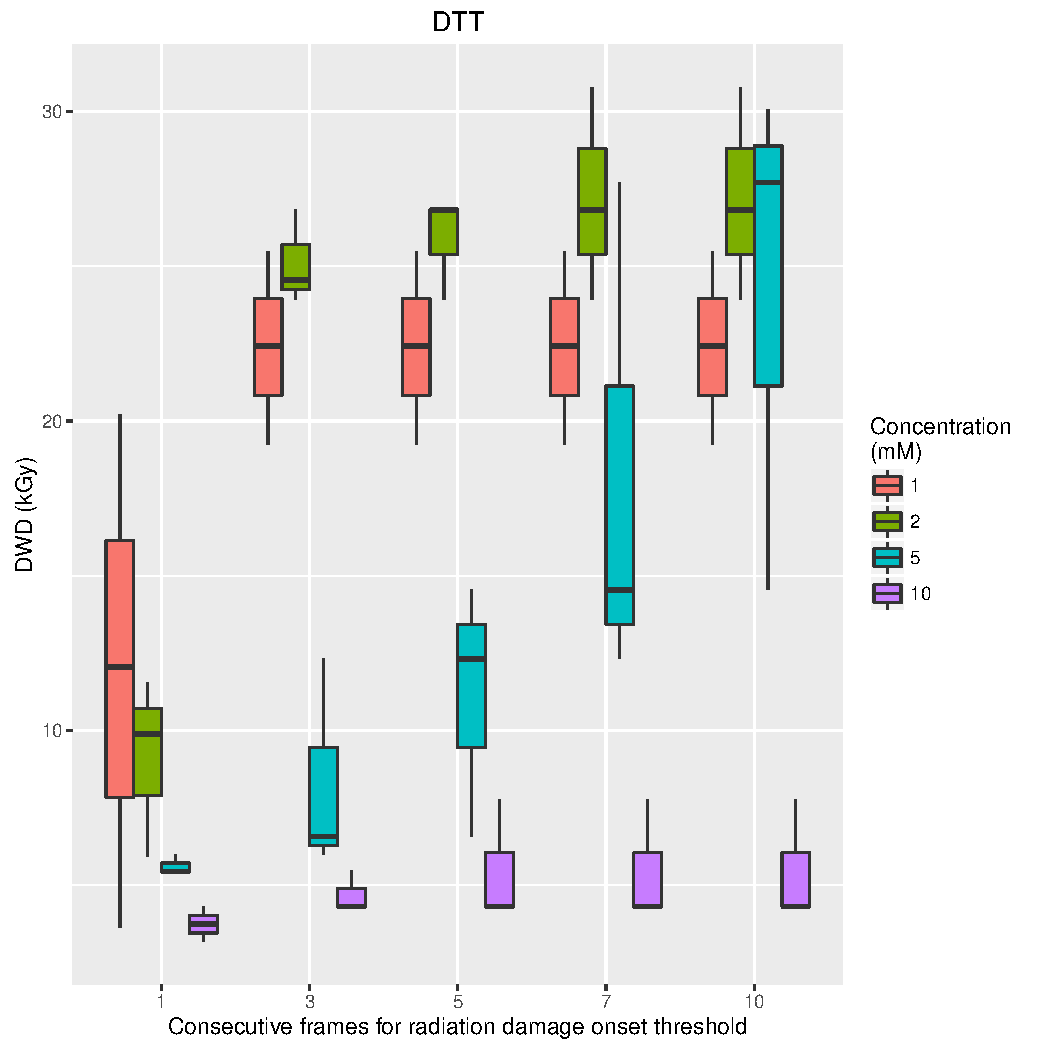
\includegraphics[width=1.0\textwidth]{figures/saxs/DTT_Num_consec_fr_comp.pdf}
    \caption{Dose at which significant radiation damage is determined to have occurred for different values of $m$ for all runs with DTT as the added radioprotectant.}
    \label{fig:Num consec frames - DTT}
\end{figure}

\subsubsection{Pairwise comparisons with all frames}
\label{subs:Pairwise comparisons with all frames}
One assumption that is made in the merging analysis is that because the first frame suffers the least amount of dose, all subsequent frames should be compared to the first frame, the \textit{reference frame}.
If instead frames were compared to a different `reference frame' would the threshold be different?
Figure~\ref{fig:First n diff frames - DTT} addresses this question by performing the analysis for the first repeat of GI sample with DTT added at 10$\,$mM concentration.
Along the $y$-axis are the frames which would be considered as the merging limit if the corresponding frame on the $x$-axis was chosen as the `reference frame'.
It can be seen that the radiation threshold value obtained using the \textit{CMD} metric is highly dependent on the reference frame.
This will greatly affect the conclusions that would be drawn from the analyses.
From Figure~\ref{fig:First n diff frames - DTT}, if the reference frame is 1, as is the case for the main analysis, then the frame at which radiation damage is considered as significant is frame 8 (DWD = 2.24$\,$kGy).
However, if the reference frame was frame 7, then the threshold frame would be 57 (DWD = 15.93\,kGy).
This value is closer to the value obtained from the \textit{BsxCuBE} metric for that run (DWD = 22.92\,kGy).
\begin{figure}
    \centering
    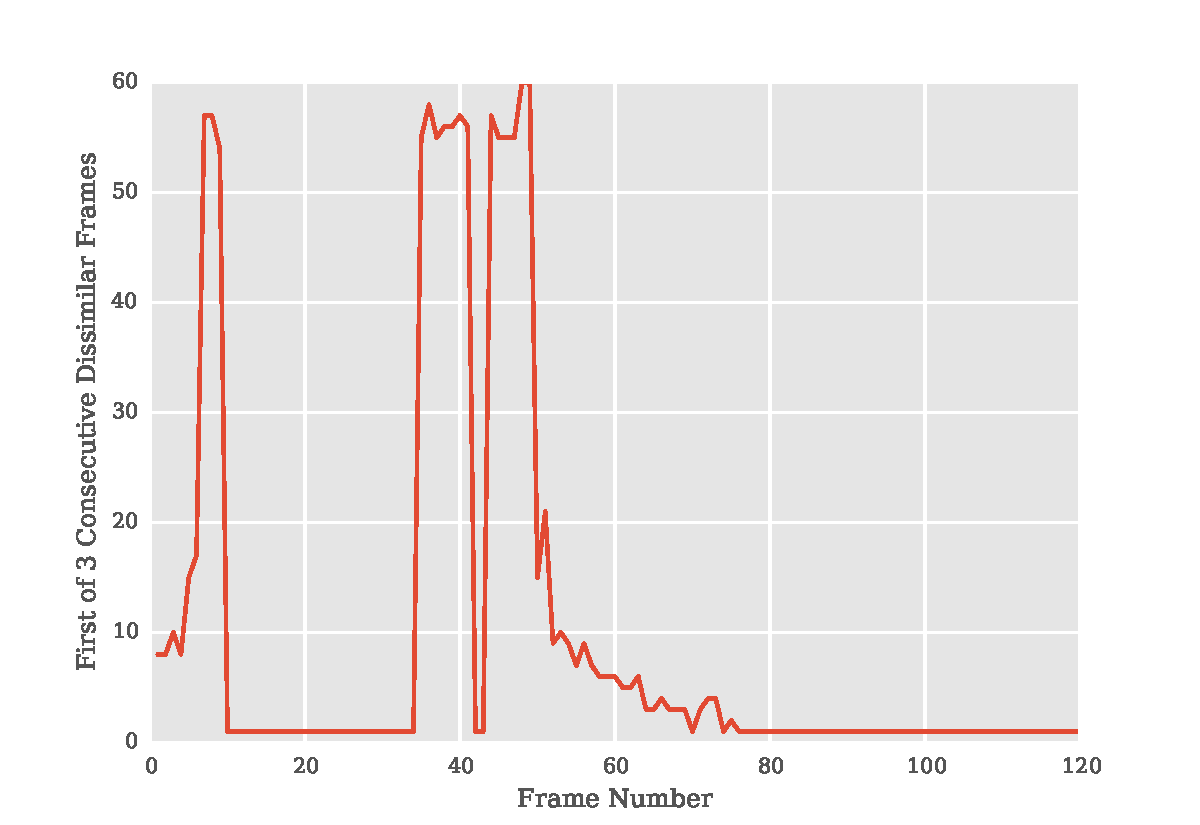
\includegraphics[width=1.0\textwidth]{figures/saxs/dtt_first_n_plot.pdf}
    \caption{Radiation damage threshold value against reference frame ($m$ = 3) for the first repeat with DTT as the added radioprotectant at a concentration of 10\,mM.}
    \label{fig:First n diff frames - DTT}
\end{figure}

The fact that performing the pairwise comparisons with different reference frames gives different results suggests that more information can be gained by analysing the results from all possible pairwise comparisons.
Figure~\ref{fig:heatmap - DTT} is a heat map showing the results from all possible pairwise frame comparisons.
The first row shows the results that were obtained using frame 1 as the reference frame.
It shows the \textit{CMD} metric highlighting frames becoming dissimilar very early on in the experiment (frame 8 out of 120).
However there is a large square region of similar frames in the top left of the map suggesting that the best results may be obtained by merging the frames from the larger region.
This region notably does not include the first frame.
The structure of this map could suggest that there are fast changes occurring in the sample early on in the experiment until a relatively stable molecular conformation is reached.
Perhaps merging frames from these different regions may result in molecular envelopes resembling the molecules in different conformations.
It may be the case that some of these states are functionally important.
\begin{figure}
    \centering
    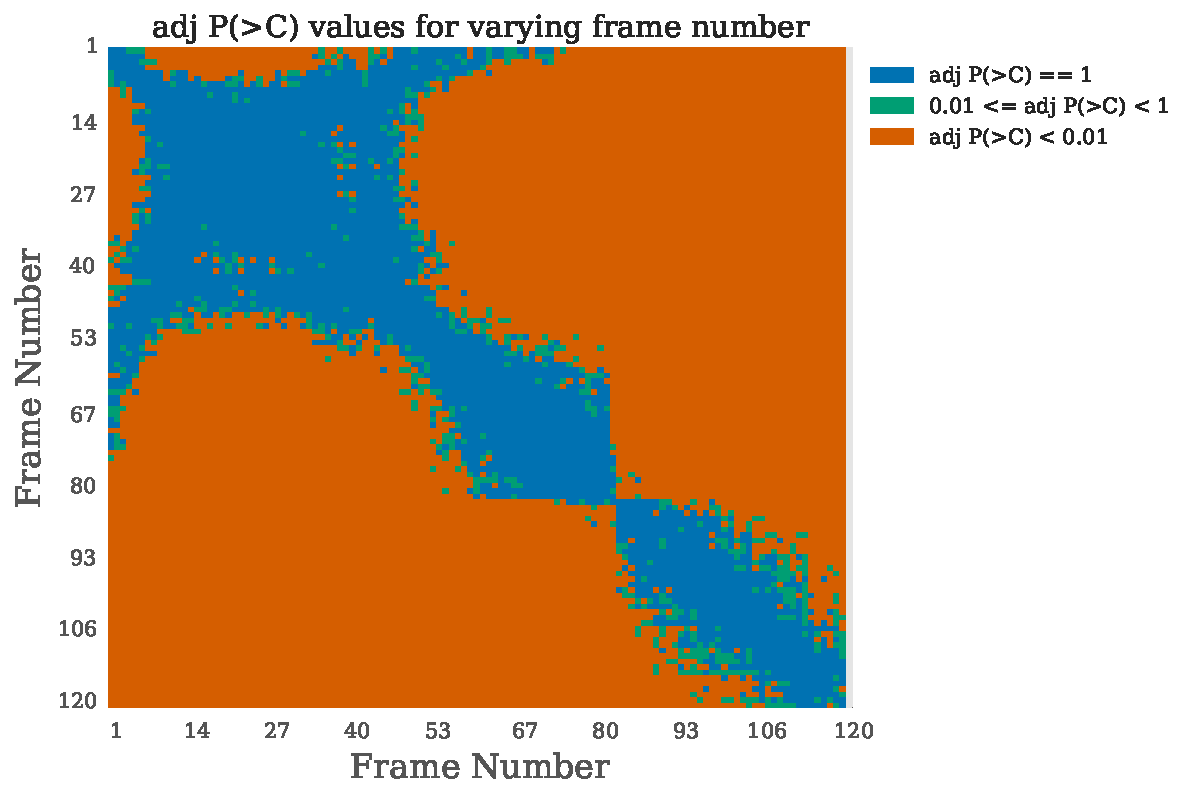
\includegraphics[width=1.0\textwidth]{figures/saxs/dtt_heatmap.pdf}
    \caption{Heat map of all possible pairwise frame comparisons for the first GI sample run with 10\,mM concentration DTT added. The $y$-axis represents the reference frame to which all other frames on the $x$-axis are compared. Blue - $P_{adj}(>C)$ = 1. Teal - $0.01 \le P_{adj}(>C)$ < 1. Orange - $P_{adj}(>C)$ < 0.01.}
    \label{fig:heatmap - DTT}
\end{figure}

\subsubsection{Using dose value and frame number as damage thresholds}
\label{subs:Using dose value and frame number as damage thresholds}
Using the dose as the metric to evaluate the efficacy of the different radioprotectants means that the results are normalised for the energy absorption of the compounds. It is sensible to ask whether this normalisation changes the conclusions that would be drawn if the frame number alone was used as the threshold metric.
Figure~\ref{fig:SAXS dose vs frame} shows the results for the 1\,mM and the 10\,mM concentrations of radioprotectants with dose value and frame number as the damage thresholds.
For the more radiation tolerant samples (ascorbate, ethylene glycol, glycerol and even DTT) there is not much difference in using either the dose or the frame number.
However for the less efficient radioprotectants (sucrose, TEMPO and trehalose) there is a significant difference.
If the frame number is used (Figures \ref{fig:SAXS frame- 1mM}, \ref{fig:SAXS frame- 10mM}) the order of the relative efficacies of those radioprotectants is not too obvious.
However if the dose value is used instead (Figures \ref{fig:SAXS dose- 1mM}, \ref{fig:SAXS dose- 10mM}) then the order becomes much clearer, particularly at 1\,mM concentration.
The spread of the threshold values for those compounds is also smaller using dose instead of frame number for the 10\,mM concentration.
\begin{figure}
    \centering
    \begin{subfigure}[b]{0.45\textwidth}
            \centering
            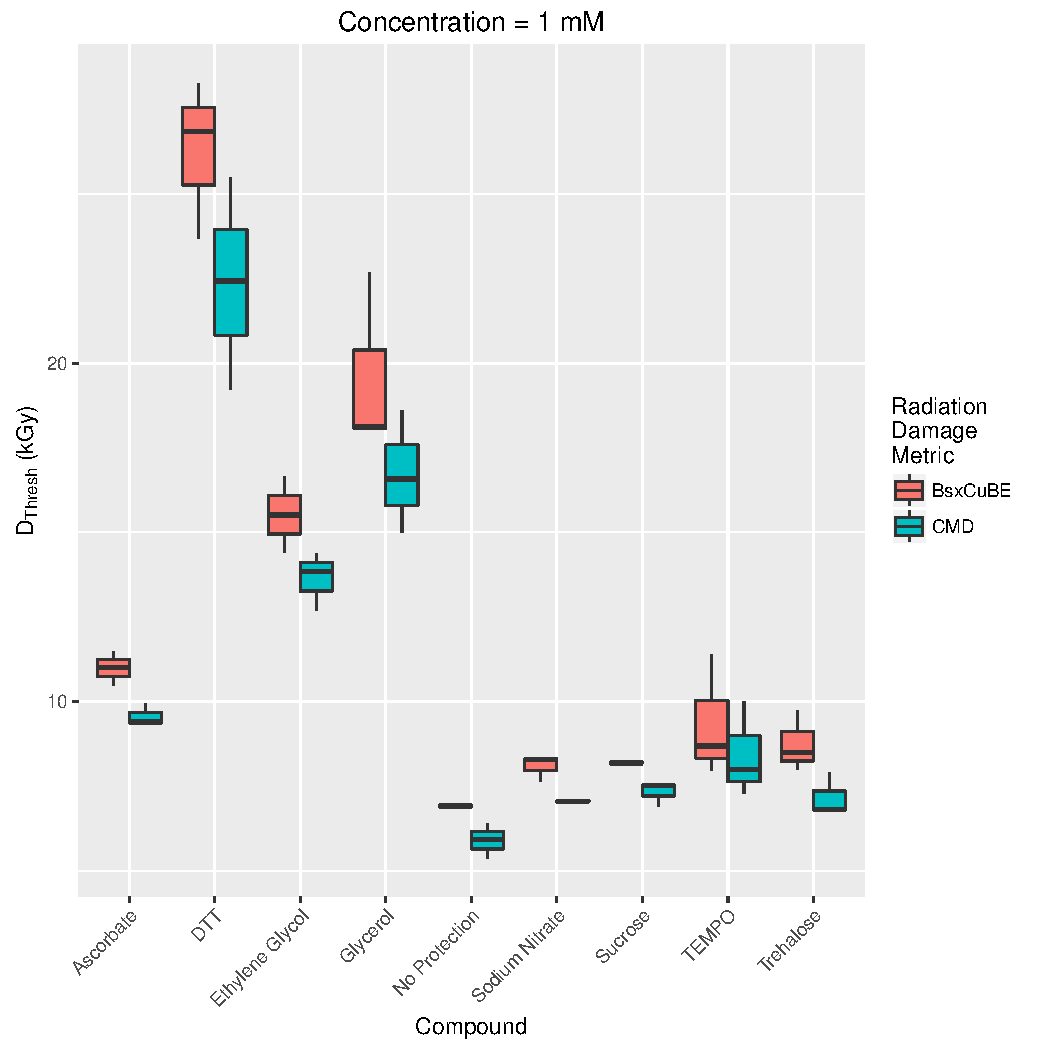
\includegraphics[width=\textwidth]{figures/saxs/Conc_1_dose.pdf}
            \caption{}
            \label{fig:SAXS dose- 1mM}
    \end{subfigure}
    \qquad
    \begin{subfigure}[b]{0.45\textwidth}
            \centering
            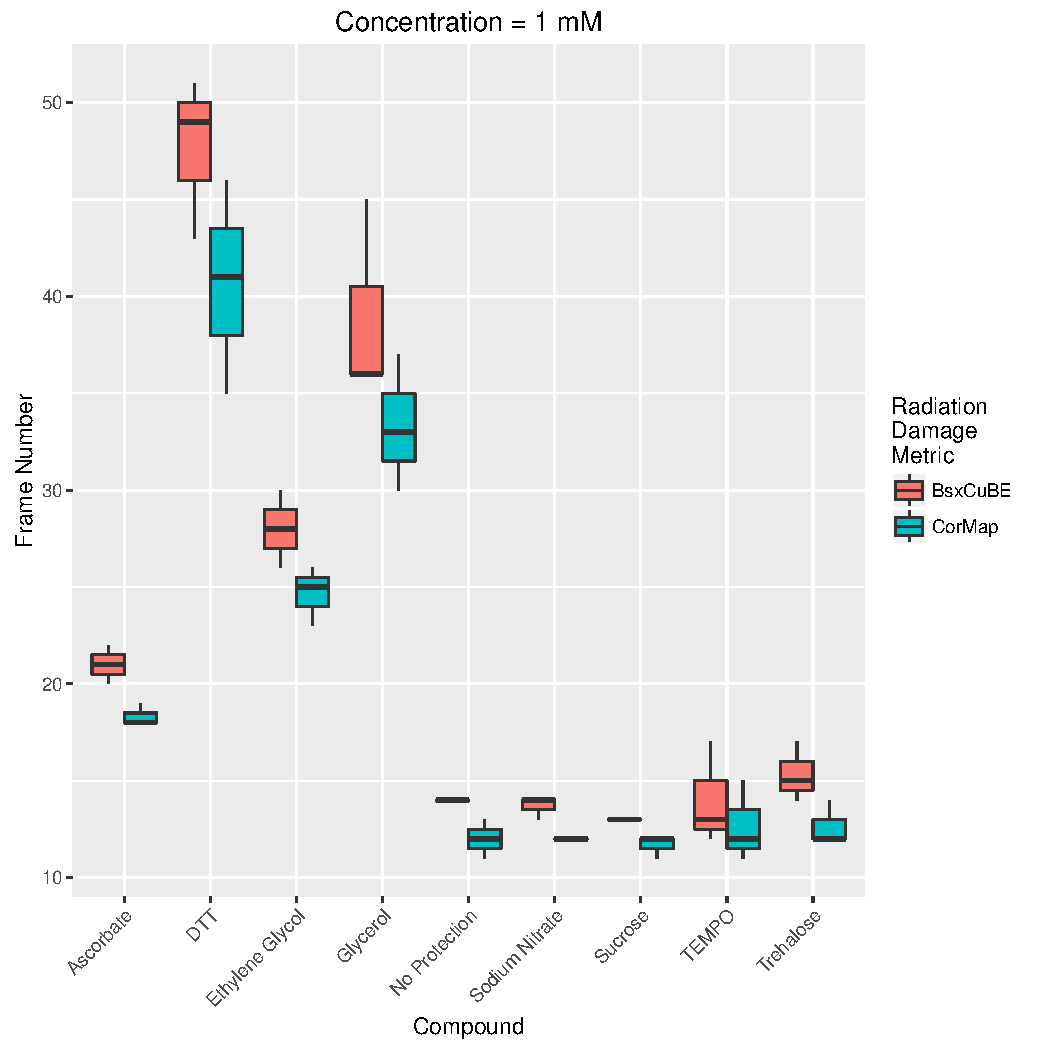
\includegraphics[width=\textwidth]{figures/saxs/Conc_1_frame_num.pdf}
            \caption{}
            \label{fig:SAXS frame- 1mM}
    \end{subfigure}
    \\
    \begin{subfigure}[b]{0.45\textwidth}
            \centering
            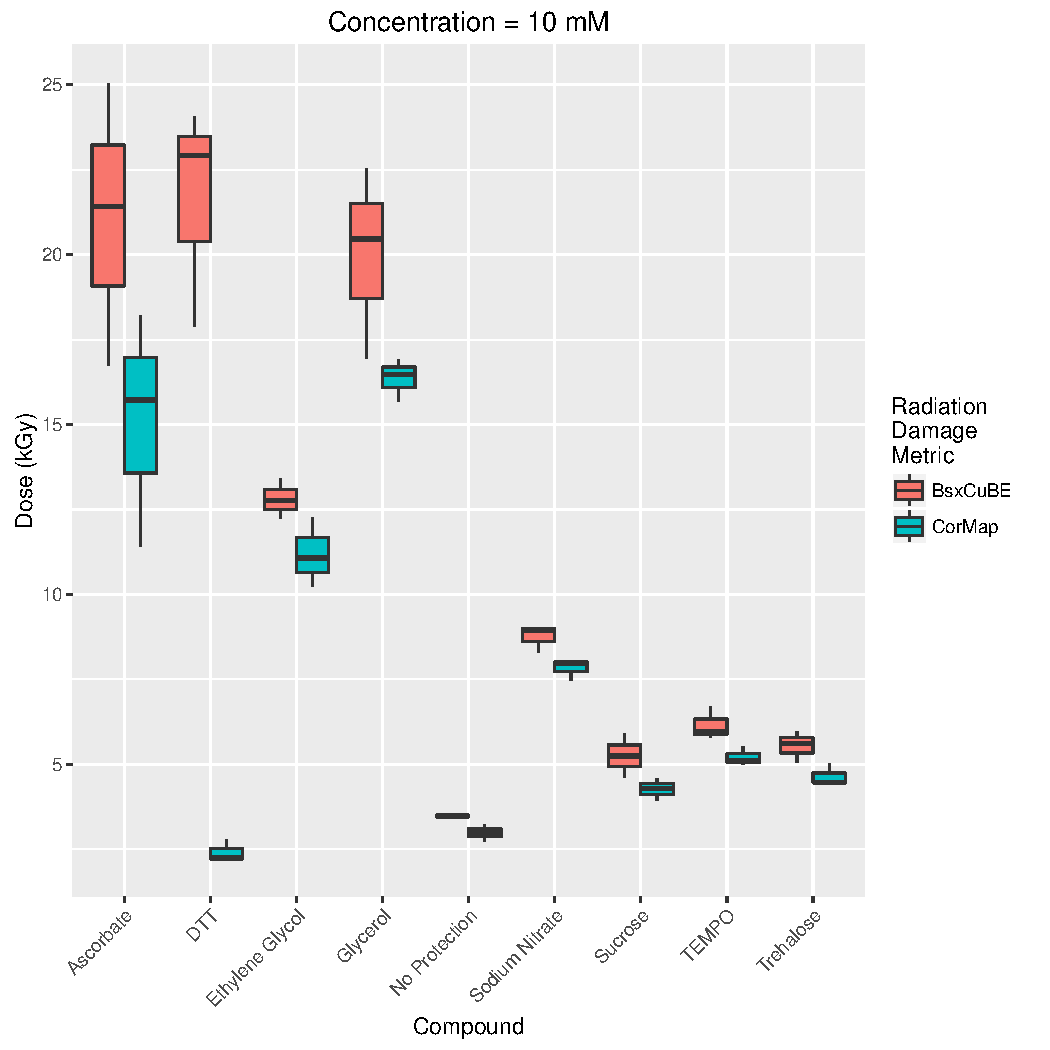
\includegraphics[width=\textwidth]{figures/saxs/Conc_10_dose.pdf}
            \caption{}
            \label{fig:SAXS dose- 10mM}
    \end{subfigure}
    \qquad
    \begin{subfigure}[b]{0.45\textwidth}
            \centering
            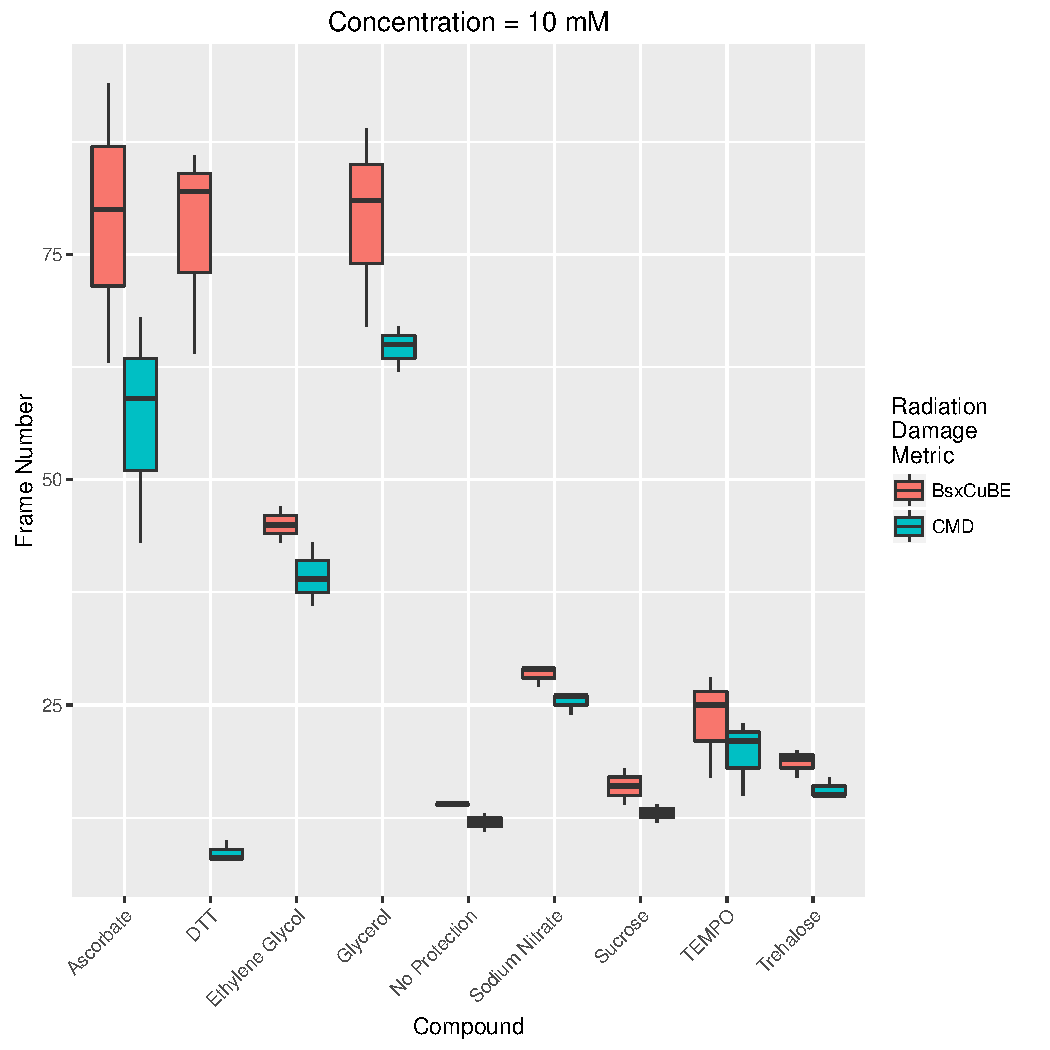
\includegraphics[width=\textwidth]{figures/saxs/Conc_10_frame_num.pdf}
            \caption{}
            \label{fig:SAXS frame- 10mM}
    \end{subfigure}
    \caption{Value at which radiation damage is considered significant. Figures on the left, [(a), (c)], show the dose value whereas those on the right, [(b), (d)], show the frame number. Each box plot is created from the threshold dose values for three different runs of the same radioprotectant compound. Pink boxes correspond to the \textit{BsxCuBE} metric, blue boxes correspond to the \textit{CMD} metric.}
    \label{fig:SAXS dose vs frame}
\end{figure}

\subsubsection{Concentration dependence}
\label{subs:Concentration dependence}
As a result of this work, a metric, RD onset ratio, was developed to assess the change in radiation tolerance in the sample with the radioprotectant added compared to no protection.
This metric is defined as the ratio of the median threshold value with added radioprotectant to the median threshold value with no protection using the \textit{CMD} metric.
Values below 1 correspond to a reduction in radiation tolerance whereas values above 1 show improved radiation tolerance.
This metric was calculated for each compound at each concentration and the results are plotted in Figure~\ref{fig:SAXS Ratio plot}.
Significant concentration dependence can be observed for several radioprotectants.
In particular, ascorbate, glycerol, and sodium nitrate all exhibit a strong positive concentration dependence i.e. the higher the concentration, the better the protection ability.
DTT exhibits the opposite behaviour.
At low concentrations DTT has the highest ratio but this decreases at the higher concentrations.
Sucrose, TEMPO and Trehalose show a very small positive dependence but even at the highest concentration (10\,mM) the RD onset ratio is less than 2.
This suggests that these radioprotectants are not very efficient at increasing the dose tolerance of the sample.
The RD onset ratio for ethylene glycol decreases as the concentration increases from 1\,mM to 5\,mM, but then there is a large increase at 10$\,$mM.
Thus the protection ability of ethylene glycol is not a simple monotonic function of the concentration.
\begin{figure}
    \centering
    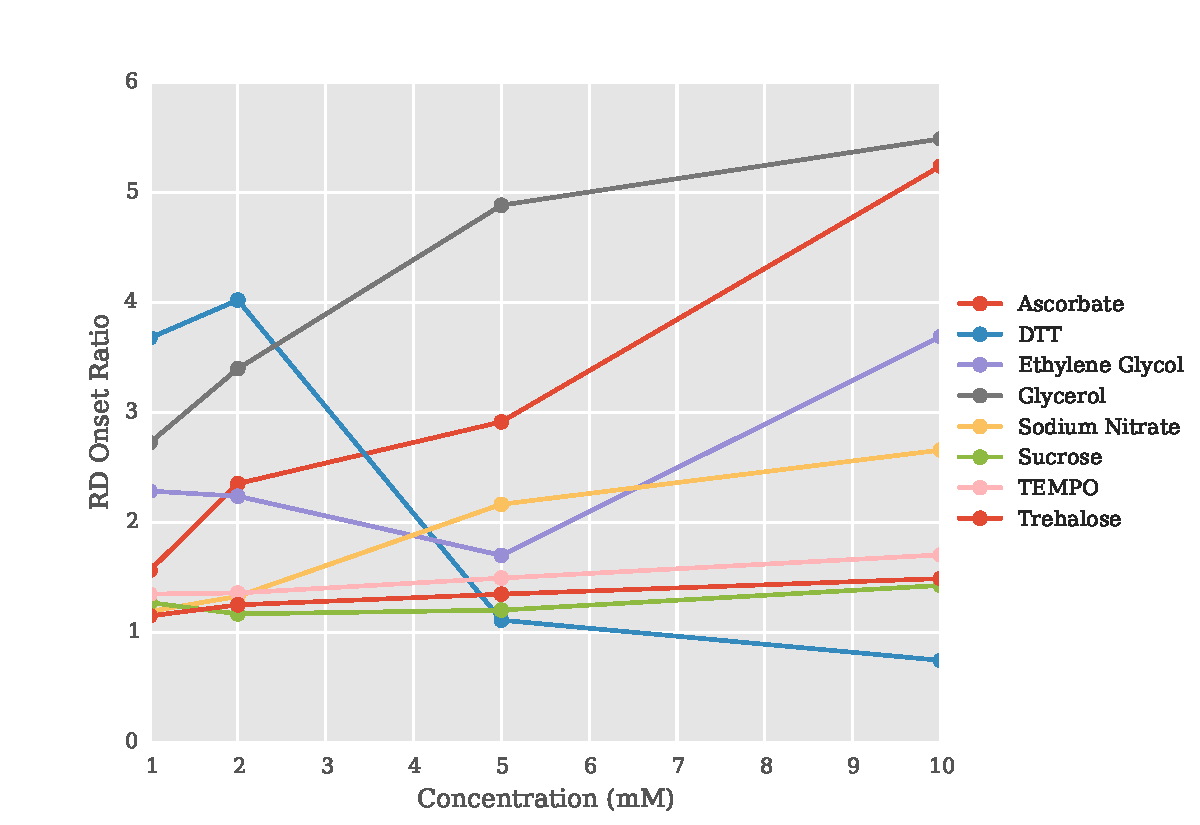
\includegraphics[width=1.0\textwidth]{figures/saxs/RatioPlots.pdf}
    \caption{Expt 2: RD onset ratio against concentration for the 8 radioprotectants.}
    \label{fig:SAXS Ratio plot}
\end{figure}

\subsubsection{Relative radioprotectant efficacy}
\label{subs:Relative radioprotectant efficacy}
The results shown in Figure~\ref{fig:SAXS Ratio plot} indicate that the most effective radioprotectant varies depending on the concentration of the compound used in the sample.
The \textit{BsxCuBE} and \textit{CMD} metrics show agreement that at low concentrations (1$\,$mM and 2$\,$mM) DTT is the most effective radioprotectant.
However at higher concentrations these metrics disagree.
At 5$\,$mM and 10$\,$mM the \textit{BsxCuBE} metric suggests that the most effective radioprotectant is still DTT.
On the otherhand, the \textit{CMD} metric suggests that the most effective radioprotectant is glycerol.
Furthermore, it also suggests that DTT is the least effective radioprotectant.
However, it is important to take into account that using a different reference frame to perform pairwise comparisons can result in different results with the \textit{CMD} metric as shown in Figures~\ref{fig:First n diff frames - DTT} and \ref{fig:heatmap - DTT}.

The \textit{CMD} metric result also disagrees with the results from experiment 1 where ethylene glycol was found to be the most effective radioprotectant at 5$\,$mM.
Furthermore, in Expt 1 ascorbate was the one of the least effective radioprotectants.
It only outperformed sucrose.
Whereas in Expt 2, ascorbate was the second most effective radioprotectant when used at a 5$\,$mM concentration.
These results could be caused by the fact that the experimental parameters were not as well characterised in the first experiment as opposed to the second.
